\section{$\nu$-SVR}

\mode<presentation>{
\begin{frame} 
    \begin{center} \huge
        \secname
    \end{center}
    \begin{center}   
    Essentially $\varepsilon$-SVR but treat $\varepsilon$ as a primal variable instead of a hyperparameter.
    \end{center}
\end{frame}
}

\subsection{Motivation}

\begin{frame}\frametitle{\subsecname~for $\nu$-SVR}

\mode<presentation>{

\begin{figure}[h]
     \centering
     \savebox{\imagebox}{
	 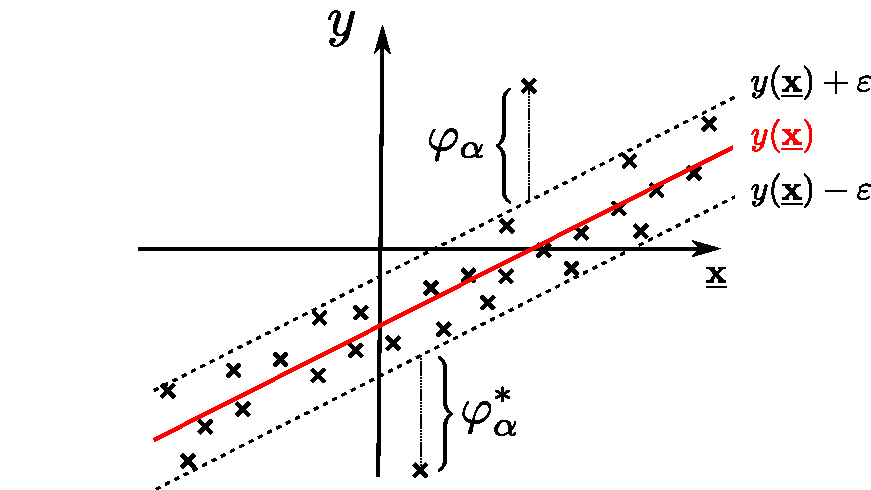
\includegraphics[width=0.4\textwidth]{img/regression_1d_linear_margin_phi}}%
     \begin{subfigure}[t]{0.4\textwidth}
         \centering
         \usebox{\imagebox}% Place largest image
     \end{subfigure}
     %\hspace{2mm}
     \begin{subfigure}[t]{0.4\textwidth}
         \centering
         \raisebox{\dimexpr.5\ht\imagebox-.5\height}{% Raise smaller image into place
         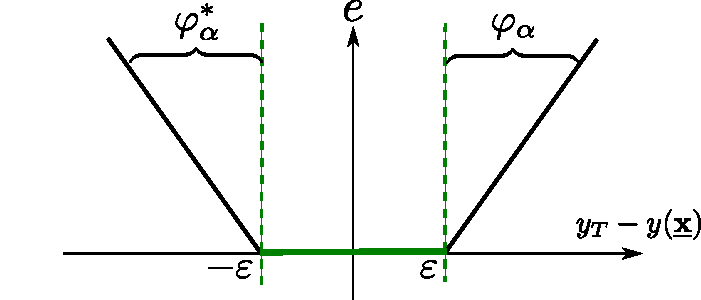
\includegraphics[width=0.99\textwidth]{img/cost_eps_phi}
         }
     \end{subfigure}
\end{figure}
}

\notesonly{
Choosing $\varepsilon$ for $\varepsilon$-SVR can be difficult as it depends on the noise in the data and this noise is unknown.
}$\varepsilon$-SVR requires treating $\varepsilon$ as a hyperparameter.
\notesonly{We therefore resort to methods such as corss-validation for choosing one value for $\varepsilon$ over another.}

$\nu$-SVR extends $\varepsilon$-SVR, by allowing the width of the ``$\varepsilon$-tube'' to adapt to the data. This is done by turning $\varepsilon$ into a \emph{primal variable}. We can then optimize w.r.t. $\varepsilon$ as we do with $\vec w, b$ and \notesonly{the set of slack variables }$\{\varphi_\alpha\}, \{\varphi_\alpha^*\}$.

\end{frame}

\subsection{Deriving the primal problem for $\nu$-SVR}

\definecolor{darkgreen}{rgb}{0,0.6,0}
\begin{frame}\frametitle{\subsecname}

\slidesonly{\vspace{-4mm}}

\begin{block}{}
     \begin{equation}
        \begin{array}{ll}
        \min_{\vec w, b,\{\varphi_\alpha\}, \{\varphi_\alpha^*\}\only<2->{, {\color{darkgreen}{\varepsilon}}}} & \frac{1}{2} \lVert \vec w \rVert_{2}^{2} + C \only<2->{\big\lbrack \nu{\color{darkgreen}\varepsilon} + } \frac{1}{p} \sum_{\alpha}^p (\varphi_\alpha + \varphi_\alpha^*) \only<2>{\big\rbrack}\\
        \text{subject to} & 
        \vec w^{\top} \vec x^{(\alpha)} + b - y_{T}^{(\alpha)} \le \varepsilon + \varphi_\alpha\\
        &
        y_{T}^{(\alpha)} - \vec w^{\top} \vec x^{(\alpha)} - b \le \varepsilon^* + \varphi_\alpha^*\\
        &\varphi_\alpha, \varphi_\alpha^* \ge 0  \qquad\qquad\qquad\qquad\quad \text{for }\alpha=1,\ldots,p \\
        &\only<2->{{\color{darkgreen}\varepsilon~\ge~0}}
        \end{array}
        \label{eq:primalnu}
     \end{equation}
     
     \slidesonly{\vspace{-3mm}}
        with $C>0$ ($C$ penalizes model error)\only<2->{, $\nu \ge 0$}
\end{block}

\pause

      \notesonly{
$\nu$-SVR extends $\varepsilon$-SVR with: 1 $\times$ new variable, 1 $\times$ new hyper-parameter, 1 $\times$ new constraint.
}

     \slidesonly{\vspace{-3mm}}

     \question{Aren't we just exchanging one hyperparameter for another? How is this better?}\\
     
\pause

     - Increased resolution of how we balance model error and model complexity. We will see that $\nu$ acts as a
     \begin{itemize}
     \item upper bound on the fraction of errors\notesonly{: $\nu \ge \frac{1}{p} \sum_{\alpha}^p (\varphi_\alpha + \varphi_\alpha^*)$}\notesonly{\\ and as a \\}
     
     \item lower bound on the fraction of SVs\notesonly{: $\nu \le \frac{\# SV}{p}$}.
     \end{itemize}
\end{frame}

\subsubsection{An intuition for $\nu$}

\begin{frame}\frametitle{\subsubsecname}

\mode<presentation>{

     \placeimage{11}{1}{img/regression_1d_linear_margin_phi_cropped_small_err}{width=3.5cm}
}

\notesonly{
We look at the part of the primal problem in which $\nu$ and $\varepsilon$ interact:
}

\slidesonly{\vspace{-20mm}}

\begin{minipage}{7.5cm}

\begin{block}{The primal problem for $\nu$-SVR (the parts where $\nu$ and $\varepsilon$ interact)}
\slidesonly{\vspace{-5mm}}
	\begingroup
	\footnotesize
     \begin{equation}
        \begin{array}{ll}
        \min_{\vec w, b,\{\varphi_\alpha\}, \{\varphi_\alpha^*\}, \varepsilon} & \\[-1mm]
        & \kern-11ex\frac{1}{2} \lVert \vec w \rVert_{2}^{2} + C \big\lbrack {\color{blue}\nu \varepsilon} + {\color{magenta}\frac{1}{p} \sum_{\alpha}^p \overbrace{(\varphi_\alpha + \varphi_\alpha^*)}^{\text{errors}}} \big\rbrack\\[2mm]
        \text{subject to} &
        \varepsilon~\ge~0\\
        \end{array}
        \label{eq:primalnuepsonly}
     \end{equation}
     
     \slidesonly{\vspace{-2mm}}
        with $C>0$, $\nu \ge 0$, $\alpha=1,\ldots,p$
     \endgroup
\end{block}
\end{minipage}

\begin{enumerate}
\item $\varepsilon = 0$:
\begin{itemize}
\item[$\Rightarrow$] All points are outside the $\varepsilon$-tube. All points are SVs, i.e. $\frac{\#\mathrm{SV}}{p}=1$.
\item[$\Rightarrow$] The \textcolor{magenta}{sum of errors} will be $> 0$
\end{itemize}
\pause
As $\varepsilon$ increases:
\begin{itemize}
\item[$\Rightarrow$] \notesonly{The term }${\color{blue}\nu\varepsilon}$ \textbf{increases} proportionally to $\nu$
\item[$\Rightarrow$] more points fall \textbf{inside} the $\varepsilon$-tube, \notesonly{leaving }a fraction $\frac{\#\mathrm{SV}}{p}$ of points \notesonly{that }are SVs\\
\item[$\Rightarrow$] \notesonly{The fraction decreases as $\varepsilon$ increases.} $\varepsilon \uparrow \;\;\leadsto\;\; \frac{\#\mathrm{SV}}{p} \downarrow$
 and the \textcolor{magenta}{sum of errors} \slidesonly{$\downarrow$}\notesonly{will \textbf{decrease}} proprtionally to $\frac{\#\mathrm{SV}}{p}$
 
\item[$\Rightarrow$] The fraction $\frac{\#\mathrm{SV}}{p} > \nu$
\end{itemize}
$\varepsilon$ stops growing as soon as the \textcolor{magenta}{sum of errors} $\corresponds~\frac{\#\mathrm{SV}}{p}$ stops decreasing. But when?

\end{enumerate}


\end{frame}

\subsection{Deriving the Lagrangian for the primal problem of $\nu$-SVR}

\subsubsection{Idenitfying the Lagrange multipliers}

\begin{frame}\frametitle{\subsecname\\ \subsubsecname}

\slidesonly{\vspace{-3mm}}

\question{Where are multipliers needed?}\\

\slidesonly{\vspace{-3mm}}

\begin{block}{The primal problem}
     \begin{equation}
        \begin{array}{lrll}
        \min_{\vec w, b,\{\varphi_\alpha\}, \{\varphi_\alpha^*\}{, {{\varepsilon}}}} && \frac{1}{2} \lVert \vec w \rVert_{2}^{2} + C {\big\lbrack \nu{\varepsilon} + } \frac{1}{p} \sum_{\alpha}^p (\varphi_\alpha + \varphi_\alpha^*) {\big\rbrack}			&\\
        \text{subject to}
        &&\vec w^{\top} \vec x^{(\alpha)} + b - y_{T}^{(\alpha)} \le \varepsilon + \varphi_\alpha		&\visible<2>{\leadsto\{\lambda_{\alpha}\}}\\
        &&y_{T}^{(\alpha)} - \vec w^{\top} \vec x^{(\alpha)} - b \le \varepsilon^* + \varphi_\alpha^*	&\visible<2>{\leadsto\{\lambda_{\alpha}^*\}}\\
        &&\varphi_\alpha \ge 0  												&\visible<2>{\leadsto\{\eta_{\alpha}\}}\\
        &&\varphi_\alpha^* \ge 0 \qquad\qquad \text{for }\alpha=1,\ldots,p 		&\visible<2>{\leadsto\{\eta_{\alpha}^*\}}\\
        &&\varepsilon \ge 0														&\visible<2>{\leadsto\delta}
        \end{array}
        %\label{eq:primalnu}
     \end{equation}
        
        with $C>0$ and $\nu \ge 0$.
\end{block}

\pause

Next: re-arrange the constraints to be in the form $f_\alpha \le 0$ to form the Lagrangian of the primal problem.

\end{frame}

\subsubsection{Re-arranging the constraints}

\begin{frame}\frametitle{\subsecname\\ \subsubsecname}

\slidesonly{\vspace{-5mm}}
\visible<1>{
Next: re-arrange the constraints to be in the form $f_\alpha \le 0$\notesonly{ to form the Lagrangian of the primal problem}:
}
\slidesonly{\vspace{-3mm}}

\mode<presentation>{
\only<1>{
\begin{block}{The primal problem}
     \begin{equation}
        \begin{array}{lrll}
        \min_{\vec w, b,\{\varphi_\alpha\}, \{\varphi_\alpha^*\}{, {{\varepsilon}}}} && \frac{1}{2} \lVert \vec w \rVert_{2}^{2} + C {\big\lbrack \nu{\varepsilon} + } \frac{1}{p} \sum_{\alpha}^p (\varphi_\alpha + \varphi_\alpha^*) {\big\rbrack}			&\\
        \text{subject to}
        &&\vec w^{\top} \vec x^{(\alpha)} + b - y_{T}^{(\alpha)} \le \varepsilon + \varphi_\alpha		&\leadsto\{\lambda_{\alpha}\}\\
        &&y_{T}^{(\alpha)} - \vec w^{\top} \vec x^{(\alpha)} - b \le \varepsilon^* + \varphi_\alpha^*	&\leadsto\{\lambda_{\alpha}^*\}\\
        &&\varphi_\alpha \ge 0  												&\leadsto\{\eta_{\alpha}\}\\
        &&\varphi_\alpha^* \ge 0 \qquad\qquad \text{for }\alpha=1,\ldots,p 		&\leadsto\{\eta_{\alpha}^*\}\\
        &&\varepsilon \ge 0														&\leadsto\delta
        \end{array}
        %\label{eq:primalnu}
     \end{equation}
        
        with $C>0$ and $\nu \ge 0$.
\end{block}
}
}
\mode<presentation>{
\only<2>{
\begin{block}{The primal problem with constraints in the form of $f_\alpha \le 0$}
     \begin{equation}
        \begin{array}{lrll}
        \min_{\vec w, b,\{\varphi_\alpha\}, \{\varphi_\alpha^*\}{, {{\varepsilon}}}} && \frac{1}{2} \lVert \vec w \rVert_{2}^{2} + C {\big\lbrack \nu{\varepsilon} + } \frac{1}{p} \sum_{\alpha}^p (\varphi_\alpha + \varphi_\alpha^*) {\big\rbrack}			&\\
        \text{subject to}
        &&\vec w^{\top} \vec x^{(\alpha)} + b - y_{T}^{(\alpha)} - \varepsilon - \varphi_\alpha	\le 0	&\leadsto\{\lambda_{\alpha}\}\\
        &&y_{T}^{(\alpha)} - \vec w^{\top} \vec x^{(\alpha)} - b - \varepsilon^* - \varphi_\alpha^*	\le 0 &\leadsto\{\lambda_{\alpha}^*\}\\
        &&- \varphi_\alpha \le 0  												&\leadsto\{\eta_{\alpha}\}\\
        && - \varphi_\alpha^* \le 0 \qquad\qquad \text{for }\alpha=1,\ldots,p 		&\leadsto\{\eta_{\alpha}^*\}\\
        && - \varepsilon \le 0														&\leadsto\delta
        \end{array}
        %\label{eq:primalnu}
     \end{equation}
        
        with $C>0$ and $\nu \ge 0$.
\end{block}
}
}

\only<3>{
\begin{block}{The primal problem with constraints in the form of $f_\alpha \le 0$}
     \begin{equation}
        \begin{array}{lrll}
        \min_{\vec w, b,\{\varphi_\alpha\}, \{\varphi_\alpha^*\}{, {{\varepsilon}}}} && \frac{1}{2} \lVert \vec w \rVert_{2}^{2} + C {\big\lbrack \nu{\varepsilon} + } \frac{1}{p} \sum_{\alpha}^p (\varphi_\alpha + \varphi_\alpha^*) {\big\rbrack}			&\\
        \text{subject to}
        &-&\{ \varphi_{\alpha} +\varepsilon+y_T^{(\alpha)} -\vec{w}^\top\vec{x}^{(\alpha)}-b \}	\le 0	&\leadsto\{\lambda_{\alpha}\}\\
        &-&\{ \varphi_{\alpha}^* 
				+\varepsilon-y_T^{(\alpha)}+\vec{w}^\top\vec{x}^{(\alpha)}+b \}	\le 0 &\leadsto\{\lambda_{\alpha}^*\}\\
        &-&\varphi_\alpha \le 0  												&\leadsto\{\eta_{\alpha}\}\\
        &-&\varphi_\alpha^* \le 0 \qquad\qquad \text{for }\alpha=1,\ldots,p 		&\leadsto\{\eta_{\alpha}^*\}\\
        &-&\varepsilon \le 0														&\leadsto\delta
        \end{array}
        %\label{eq:primalnu}
     \end{equation}
        
        with $C>0$ and $\nu \ge 0$.
\end{block}
}

\end{frame}

\begin{frame}\frametitle{\subsecname}

\slidesonly{\vspace{-5mm}}

\begin{equation}
\left.\begin{aligned}
				L(\underbrace{\vec{w},b,\{\varphi_{\alpha}\},\{\varphi_{\alpha}^*\},\varepsilon}_{\text{primal variables}},
				\underbrace{\{\lambda_{\alpha}\}, \{\lambda_{\alpha}^*\},\{\eta_{\alpha}\},\{\eta_{\alpha}^*\},\delta}_{\mathclap{\text{dual variables (Lagrange multipliers)}}})\\
				= \smallfrac{1}{2} \lVert\vec{w}\rVert^2_2+C \Big\lbrack \nu \varepsilon 
					+ \smallfrac{1}{p} \sum_{\alpha=1}^p(\varphi_{\alpha}
					+\varphi_{\alpha}^*) \Big\rbrack \\
				-\sum_{\alpha=1}^p \lambda_{\alpha} \{\varphi_{\alpha}
				+\varepsilon+y_T^{(\alpha)}
				-\vec{w}^\top\vec{x}^{(\alpha)}-b \}  \\
				-\sum_{\alpha=1}^p \lambda_{\alpha}^* \{\varphi_{\alpha}^* 
				+\varepsilon-y_T^{(\alpha)}+\vec{w}^\top\vec{x}^{(\alpha)}+b \} \\ 
				-\sum_{\alpha=1}^p \eta_{\alpha} \varphi_{\alpha} 
				- \sum_{\alpha=1}^p \eta_{\alpha}^* \varphi_{\alpha}^* 
				- \delta \varepsilon
			\end{aligned}\right.
\end{equation}

with $\{\lambda_{\alpha}\}, \{\lambda_{\alpha}^*\},\{\eta_{\alpha}\},\{\eta_{\alpha}^*\},\delta \ge 0$

\end{frame}

